



\chapter{Information chiffrée}

\section{Proportion et pourcentage}

\subsection{Proportion d'une sous-population}

\begin{Exemple}
\begin{minipage}[c]{0.7\linewidth}
Sur les $150$ élèves inscrits en classe de seconde,
$36$ d'entre eux sont externes.
\vspace{0.1cm}

\ligne

\ligne

\ligne

\ligne

\ligne

\ligne

\ligne

\ligne

\ligne

\end{minipage} \hfill
\begin{minipage}[c]{0.25\linewidth}
\begin{center}
\begin{tikzpicture}[scale=.75] 
\def\A{(2,2) circle[x radius=3cm, y radius=2cm]} ;
\def\B{(2.5,1.8) circle[x radius=1.3cm, y radius=1cm]} ;
\draw[Couleur1] \A ;
\draw[Couleur1] (0.9,3.3) node{Seconde} ; \draw[Couleur10] \B ;
\draw[Couleur10] (2.4,2) node{Externe} ;  
\draw[Couleur1] (0.9,2.7) node{$150$} ;
\draw[Couleur10] (2.4,1.4) node{$36$} ; 
\end{tikzpicture} 
\end{center}
\end{minipage}

\end{Exemple}

\subsection{Pourcentage d'un nombre}

\begin{Exemple}
Parmi les $150$ élèves de seconde, $12\%$ ont choisi comme deuxième langue l'allemand. Combien cela représente-il d'élève ?
\vspace{0.1cm}

\ligne

\end{Exemple}

\begin{Méthode}Associer effectif, proportion et pourcentage. \\
Une société de $75$ employés compte $12 \%$ de cadres et le reste d'ouvriers. $35$ employés de cette société sont des femmes et $5$ d'entre elles sont cadres. 
\begin{enumerate}
\item Calculer l'effectif des cadres.

\ligne

\item Calculer la proportion de femmes dans cette société.

\ligne

\ligne
     
\item Calculer la proportion, en $\%$, de cadres parmi les femmes. Les femmes cadres sont-elles sous ou sur-représentées dans cette société ?

\ligne

\ligne

\ligne

\ligne

\end{enumerate}
\end{Méthode}

\newpage

\subsection{Proportions échelonnées}

\begin{Exemple}
\begin{minipage}[c]{0.5\linewidth}
Dans un car, il y a ${\color{Couleur1}{35\%}}$ de scolaires. Parmi les scolaires, ${\color{Couleur10}{60\%}}$ sont des filles. \\
L'ensemble ${\color{Couleur10}{F}}$ est inclus dans l'ensemble ${\color{Couleur1}{S}}$ et on a \\
${\color{Couleur10}{p_F}}={\color{Couleur10}{60\%}}$ de ${\color{Couleur1}{S}}$.\\
L'ensemble ${\color{Couleur1}{S}}$ est inclus dans l'ensemble $CAR$ et
on a \\
${\color{Couleur1}{p_S}}={\color{Couleur1}{35\%}}$ de $CAR$.\\
La proportion de scolaires filles dans le $CAR$ est donc égale à : 

\ligne

\end{minipage} \hfill
\begin{minipage}[c]{0.5\linewidth}
\begin{center} 
\begin{tikzpicture}[scale=.75] 
\def\C{ (-2,-1) rectangle (6,5) };
\def\A{(2,2) circle[x radius=3cm, y radius=2cm]} ;
\def\B{(2.3,2.3) circle[x radius=2cm, y radius=1cm]} ;
\draw[Couleur1] \A ;
\draw[Couleur1] (3.5,0) node{$S$} ; \draw[Couleur10] \B ;
\draw[Couleur10] (4.5,1.7) node{$F$} ; 
\draw (0,-0.5) node{$CAR$} ; \draw \C;
\draw[Couleur1] (2,0.8) node{$35\% \text{ de } CAR$} ;
\draw[Couleur10] (2.3,2.3) node{$60\% \text{ de } S$} ; 
\end{tikzpicture} 
\end{center}
\end{minipage}

\end{Exemple}

\begin{Propriété} $ $ \\
\begin{minipage}[c]{0.5\linewidth}
$A\subset B$ et $B \subset C$.\\
$p_1$ est la proportion de $A$ dans $B$.\\
$p_2$ est la proportion de $B$ dans $C$.\\
Alors $p=p_1\times p_2$ est la proportion de $A$ dans $C$.
\end{minipage} \hfill
\begin{minipage}[c]{0.4\linewidth}
\begin{center} 
\begin{tikzpicture}[scale=.4] 
\def\R{ (0,0) circle[x radius=5cm, y radius=3.5cm] };
\def\Q{ (0,0) circle[x radius=3.5cm, y radius=2.3cm] };
\def\D{ (0,0) circle[x radius=2cm, y radius=1.1cm] };

\begin{scope}
\clip \R ;
\fill[Couleur11!20] \R ;
\end{scope}

\begin{scope}
\clip \R ;
\fill[Couleur10!20] \Q;
\end{scope}

\begin{scope}
\clip \Q ;
\fill[Couleur1!20] \D;
\end{scope}

\draw[Couleur11] \R ;
\draw[Couleur10] \Q ;
\draw[Couleur1] \D ;

\draw[Couleur11] (4.5,2.8) node{${C}$} ; 
\draw[Couleur10] (3.5,1.5) node{${B}$} ; 
\draw[Couleur1] (2.5,0.5) node{${A}$} ; 
\end{tikzpicture} 
\end{center}
\end{minipage}
\end{Propriété}

\begin{Méthode}Calculer des pourcentages de pourcentages. \\
Sur $67$ millions d'habitants en France, $66 \%$ de la population est en âge de travailler ($15$- $64$ ans).\\
La population active représente $70 \%$ de la population en âge de travailler.
\begin{enumerate}
\item Calculer la proportion de population active par rapport à la population totale.

\ligne

\ligne

\ligne

\ligne

\ligne

\ligne

\ligne

\ligne

\item Combien de français compte la population active ?

\ligne

\ligne

\end{enumerate}
\end{Méthode}

\newpage

\section{Évolution exprimée en pourcentage}

\subsection{Calculer une évolution}

\begin{Propriétés} $ $\\
\begin{itemize}[label=\textcolor{Couleur2}{$\bullet$}]
\item Augmenter une valeur de $t\%$ revient à la multiplier par $1+\dfrac{t}{100}$.
\item Diminuer une valeur de $t\%$ revient à la multiplier par $1-\dfrac{t}{100}$.
\item $1+\dfrac{t}{100}$ et $1-\dfrac{t}{100}$ sont appelés les {\bf{coefficients multiplicateurs}}. 
\end{itemize}
\end{Propriétés}

\begin{Remarque}
Si on augmente une valeur $V_0$ de $t\%$ alors sa valeur $V_1$ après augmentation est égale à : $V_1=V_0+V_0\times \dfrac{t}{100}=V_0\left(1+\dfrac{t}{100}\right)$\\
Si on diminue une valeur $V_0$ de $t\%$ alors sa valeur $V_1$ après diminution est égale à : $V_1=V_0-V_0\times \dfrac{t}{100}=V_0\left(1-\dfrac{t}{100}\right)$
\end{Remarque}

\begin{Exemples}
\leavevmode\vspace{-\baselineskip}
\begin{itemize}
\item Le prix d'un survêtement est de $49$€. Il augmente de $8\%$. \\
Son nouveau prix est égal à : \ligne

\item Le prix d'un polo est de $21$€. Il est soldé de $20\%$. \\
Son nouveau prix est égal à : \ligne
\end{itemize}
\end{Exemples}

\subsection{Calculer un taux d'évolution}

\begin{Définition}
On considère une valeur $V_0$ qui subit une évolution pour arriver à une valeur $V_1$.\\
Le {\bf{taux d'évolution}} est égal à : $t=\dfrac{V_1-V_0}{V_0}$.
\end{Définition}

\begin{Remarque}
\leavevmode\vspace{-\baselineskip}
\begin{itemize}
\item Si $t>0$, l'évolution est une augmentation.
\item Si $t<0$, l'évolution est une diminution.
\end{itemize}
\end{Remarque}

\begin{Exemples}
\leavevmode\vspace{-\baselineskip}
\begin{itemize}
\item La population d'un village est passé de $8\,500$ à $10\,400$ entre $2008$ et $2012$. De combien de pourcentage a-t-elle augmenté ?

\ligne

\ligne

\ligne

\item Le prix d'une console passe de $399$€ à  $349$€. De combien de pourcentage a-t-il diminué ?

\ligne

\ligne

\ligne

\end{itemize}
\end{Exemples}

\newpage

\subsection{Évolutions successives}

\begin{Propriété}
\begin{itemize}[label=\textcolor{Couleur2}{$\bullet$}]
\item Lors de $n$ évolutions successives à des taux $t_1$,$t_2,\ldots,t_n$ (augmentations et/ou diminutions) entre une valeur $V_0$ et une valeur $V_n$, on appelle  {\bf{taux d'évolution global}} le taux noté $T$, qu'il faut appliquer  à la valeur $V_0$ pour obtenir la valeur $V_n$.

\begin{center}
\begin{tikzpicture}
\node[draw] (A) at (0,0) {$V_0$};
\draw (1,1) node {$\times (1+t_1)$};
\node[draw] (B) at (2,0) {$V_1$};
\draw (3,1) node {$\times (1+t_2)$};
\node[draw] (C) at (4,0) {$V_2$};

\node[draw] (D) at (6,0) {$V_{\ldots}$};

\node[draw] (E) at (8,0) {$V_{n-1}$};
\draw (9,1) node {$\times (1+t_n)$};
\node[draw] (F) at (10,0) {$V_{n}$};
\draw[Couleur11] (12,1) node {coefficients};
\draw[Couleur11] (12,0.5) node {multiplicateurs};

\draw (5,-2) node {$\times (1+T)$};
\draw[Couleur11] (8.5,-2) node {: coefficient multiplicateur global};

\draw[->,>=latex] (A.north) to[bend left=45] (B.north) ;
\draw[->,>=latex] (B.north) to[bend left=45] (C.north);
\draw[->,>=latex] (C.north) to[bend left=45] (D.north);
\draw[->,>=latex] (D.north) to[bend left=45] (E.north);
\draw[->,>=latex] (E.north) to[bend left=45] (F.north);
\draw[->,>=latex] (A.south) to[bend left=-25] (F.south);
\end{tikzpicture}
\end{center}

\item Le {\bf{taux d'évolution global}} $T$ est donc tel que $(1+T)=(1+t_1)(1+t_2)\ldots(1+t_n)$

\begin{minipage}[c]{0.6\linewidth}
\item Dans le cas de deux évolutions successives, en nommant
respectivement $t_1$ et $t_2$ les taux de la première et de la seconde évolution. Alors la quantité $V_0$ a subi une évolution globale de taux $T$ tel que $1+T=(1+t_1)\times (1+t_2)$ .
\end{minipage} \hfill
\begin{minipage}[c]{0.4\linewidth}
\begin{center}
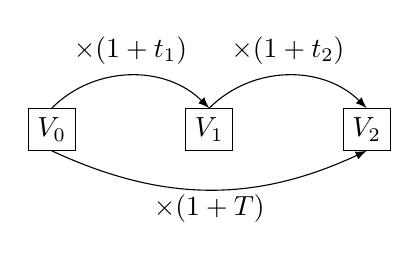
\begin{tikzpicture}
\node[draw] (A) at (0,0) {$V_0$};
\draw (1,1) node {$\times (1+t_1)$};
\node[draw] (B) at (2,0) {$V_1$};
\draw (3,1) node {$\times (1+t_2)$};
\node[draw] (C) at (4,0) {$V_2$};

\draw (2,-1) node {$\times (1+T)$};

\draw[->,>=latex] (A.north) to[bend left=45] (B.north) ;
\draw[->,>=latex] (B.north) to[bend left=45] (C.north);
\draw[->,>=latex] (A.south) to[bend left=-25] (C.south);
\end{tikzpicture}
\end{center}
\end{minipage}
\end{itemize}
\end{Propriété}

\begin{Exemple}
Un site marchand décide d'augmenter tous ses prix de $20 \%$ avant Noël, puis de les baisser de $25 \%$ pour les soldes de mi-janvier.
À la mi-janvier combien coûte un jouet qui coûtait $80$€ en octobre ? 
\vspace{0.1cm}

\ligne

\ligne

\ligne

\ligne

\end{Exemple}

\subsection{Évolutions réciproques}

\begin{Propriété} $ $ \\
\begin{minipage}[c]{0.7\linewidth}
Une quantité $V_0$ subit une évolution au taux $t$ pour obtenir une quantité $V_1$. On désigne par $t'$ le taux d'évolution réciproque de $V_1$ à $V_0$ . Alors $1+t '=\dfrac{1}{1+t}$.
\end{minipage} \hfill
\begin{minipage}[c]{0.4\linewidth}
\begin{center}
\begin{tikzpicture}
\node[draw] (A) at (0,0) {$V_0$};
\draw (1,1) node {$\times (1+t)$};
\node[draw] (B) at (2,0) {$V_1$};

\draw (1.5,-1) node {$\times (1+t')=\dfrac{1}{1+t}$};

\draw[->,>=latex] (A.north) to[bend left=45] (B.north) ;
\draw[<-,>=latex] (A.south) to[bend left=-25] (B.south);
\end{tikzpicture}
\end{center}
\end{minipage}
\end{Propriété}

\begin{Exemple}
Une station essence augmente tous ses tarifs de $11\%$ avant un long week-end. Le prix du SP95 E10 est de $1,359$€. Combien coûtait-il avant l'augmentation ? 
\vspace{0.1cm}

\ligne

\ligne

\ligne

\ligne

\end{Exemple}

\bigskip

\newpage

\section*{Exercices - Information chiffrée}
\addcontentsline{toc}{section}{Exercices}
{\setlength{\columnseprule}{0pt}
\setcounter{NumEx}{1}


\subsection*{Proportion et pourcentages}


% @see : https://coopmaths.fr/alea?uuid=ae913&id=2S10-1&n=2&d=10&s=1&alea=qIx7&cd=1&cols=1
\begin{Exercice}
\leavevmode\vspace{-\baselineskip}
\begin{enumerate}
	\item Écrire sous la forme d'une écriture fractionnaire de dénominateur $100$, puis sous la forme d'un pourcentage. $8{,}6=\makebox[.08\linewidth]{\dotfill}=\makebox[.08\linewidth]{\dotfill}\,\%$
	\item Écrire sous la forme d'une écriture fractionnaire de dénominateur $100$, puis sous la forme d'un pourcentage. $0{,}066=\makebox[.08\linewidth]{\dotfill}=\makebox[.08\linewidth]{\dotfill}\,\%$
\end{enumerate}
\end{Exercice}

% @see : https://coopmaths.fr/alea?uuid=ae913&id=2S10-1&n=2&d=10&s=2&alea=Og39&cd=1&cols=1
\begin{Exercice}
\leavevmode\vspace{-\baselineskip}
\begin{enumerate}
	\item Écrire sous forme décimale, puis sous la forme d'une écriture fractionnaire de dénominateur $100$.\\
$7{,}3\,\%=\makebox[.08\linewidth]{\dotfill}=\makebox[.08\linewidth]{\dotfill}$
	\item Écrire sous forme décimale, puis sous la forme d'une écriture fractionnaire de dénominateur $100$.\\
$0{,}52\,\%=\makebox[.08\linewidth]{\dotfill}=\makebox[.08\linewidth]{\dotfill}$\\
\end{enumerate}
\end{Exercice}

% @see : https://coopmaths.fr/alea?uuid=ae913&id=2S10-1&n=2&d=10&s=3&alea=vt2d&cd=1&cols=1
\begin{Exercice}
\leavevmode\vspace{-\baselineskip}
\begin{enumerate}
	\item Écrire sous forme décimale, puis sous la forme d'un pourcentage. $\dfrac{7}{8}=\makebox[.08\linewidth]{\dotfill}=\makebox[.08\linewidth]{\dotfill}\,\%$
	\item Écrire sous forme décimale, puis sous la forme d'un pourcentage. $\dfrac{21}{25}=\makebox[.08\linewidth]{\dotfill}=\makebox[.08\linewidth]{\dotfill}\,\%$
\end{enumerate}
\end{Exercice}



% @see : https://coopmaths.fr/alea?uuid=612a5&id=2S10-2&n=2&d=10&s=2&alea=l4EE&cd=1&cols=1
\begin{Exercice}
\leavevmode\vspace{-\baselineskip}
\begin{enumerate}
	\item Une réserve de protection d'oiseaux contient $2\,000$ individus d'oiseaux. On dénombre $280$ pics noirs. \\Calculer la proportion en pourcentage de pics noirs dans la réserve.
	\item Parmi les $2\,140$ spectateurs d'un concert, $963$ ont moins de $18$ ans. \\Calculer la proportion des personnes mineures dans le public en pourcentage.
\end{enumerate}
\end{Exercice}

% @see : https://coopmaths.fr/alea?uuid=612a5&id=2S10-2&n=2&d=10&s=1&alea=D835&cd=1&cols=1
\begin{Exercice}
\leavevmode\vspace{-\baselineskip}
\begin{enumerate}
	\item Le cadeau commun que nous souhaitons faire à Kaïs coûte $150$ €. Je participe à hauteur de $6~\%$ du prix total. Combien ai-je donné pour le cadeau de Kaïs ?
	\item Une réserve de protection d'oiseaux contient $1\,300$ individus d'oiseaux. On dénombre $25~\%$ de pipits farlouse. Quel est le nombre de pipits farlouse ?
\end{enumerate}
\end{Exercice}

% @see : https://coopmaths.fr/alea?uuid=612a5&id=2S10-2&n=2&d=10&s=3&alea=HnKG&cd=1&cols=1
\begin{Exercice}
\leavevmode\vspace{-\baselineskip}
\begin{enumerate}
	\item Lors d'un concert, il y a $1\,458$ spectateurs de plus de $60$ ans, ce qui représente $54~\%$ du public. \\Combien de spectateurs ont assisté au concert ?
	\item Pour le cadeau de Nadia, j'ai donné $24$ €. Cela représente $20~\%$ du prix total du cadeau. \\Quel est le montant du cadeau ?
\end{enumerate}
\end{Exercice}

\newpage

\begin{Exercice} %3

 \begin{minipage}[t]{\linewidth}Dans un lycée, on compte $350$ élèves en classe de première dont $50 \,\%$ sont des garçons et $60 \,\%$ sont dans une filière générale. \\
      De plus, $26 \,\%$ des élèves sont des garçons en première générale.\\ Compléter le tableau suivant :
      
\begin{center}

\medskip
$\renewcommand{\arraystretch}{1}
\begin{array}{|c|c|c|c|}
\arrayrulecolor{Couleur6} \hline
 ~ &   \text{Garçons} &   \text{Filles} &   \text{Total}\\
\hline
  \text{Première générale} &  &  & \\
\hline
  \text{Première technologique} &  &  & \\
\hline
  \text{Total} &  &  & \\
\hline
\end{array}
\renewcommand{\arraystretch}{1}$

\end{center}
\end{minipage}\\

\end{Exercice}



\begin{Exercice} %4

 \begin{minipage}[t]{\linewidth}Dans un lycée, on compte $250$ élèves en classe de première.\\
        Ils sont répartis selon le tableau suivant :
\begin{center}
\medskip
 $\renewcommand{\arraystretch}{1}
\begin{array}{|c|c|c|c|}
\arrayrulecolor{Couleur6} \hline
  ~ &   \text{Garçons} &   \text{Filles} &   \text{Total}\\
\hline
  \text{Filière générale} & 70 & 55 & 125\\
\hline
  \text{Filière technologique} & 30 & 95 & 125\\
\hline
  \text{Total} & 100 & 150 & 250\\
\hline
\end{array}
\renewcommand{\arraystretch}{1}$
\end{center}

\medskip
\textbf {a.}   Quelle est la proportion de filles en première technologique parmi les élèves de ce lycée ?\\Sous la forme d'une fraction : $\ldots$\\Sous la forme d'un pourcentage (arrondir à l'unité si besoin) : $\ldots\,\%$

\medskip
\textbf {b.}  Quelle est la proportion de filles en première technologique parmi les élèves en première technologique ?\\Sous la forme d'une fraction : $\ldots$\\Sous la forme d'un pourcentage (arrondir à l'unité si besoin) : $\ldots\,\%$

\medskip
\textbf {c.}   Quelle est la proportion de filles en première technologique parmi les filles ?\\Sous la forme d'une fraction : $\ldots$\\Sous la forme d'un pourcentage (arrondir à l'unité si besoin) : $\ldots\,\%$\end{minipage}\\

\end{Exercice}

\begin{Exercice} %6
Dans un lycée,  $35\,\%$ des lycéens sont en classe de première et  $15{,}05\,\%$ des lycéens sont en première technologique.\\
              Quel est le pourcentage d'élèves en première technologique parmi les élèves de première ?\\

\end{Exercice}

\subsection*{Évolution}


\begin{Exercice} %5
Compléter.
\vspace{-0.5cm}
\begin{multicols}{2}
\begin{enumerate}
	\item \begin{minipage}[t]{\linewidth}Multiplier par $0{,}88$ revient à ...\end{minipage}
	\item \begin{minipage}[t]{\linewidth}Augmenter de $21~\%$ revient à multiplier par ...\end{minipage}
	\item \begin{minipage}[t]{\linewidth}Multiplier par $1{,}15$ revient à ...\end{minipage}
	\item \begin{minipage}[t]{\linewidth}Diminuer de $80~\%$ revient à multiplier par ...\end{minipage}
	\item \begin{minipage}[t]{\linewidth}Multiplier par $0{,}92$ revient à ...\end{minipage}
	\item \begin{minipage}[t]{\linewidth}Multiplier par $1{,}17$ revient à ...\end{minipage}
	\item \begin{minipage}[t]{\linewidth}Augmenter de $3~\%$ revient à multiplier par ...\end{minipage}
	\item \begin{minipage}[t]{\linewidth}Diminuer de $18~\%$ revient à multiplier par ...\end{minipage}
\end{enumerate}
\end{multicols}
\end{Exercice}


\newpage




% @see : https://coopmaths.fr/alea?uuid=12444&id=2S11-2&n=3&d=10&s=1&alea=TQG8&cd=1&cols=1
\begin{Exercice}
\leavevmode\vspace{-\baselineskip}
\begin{enumerate}
	\item Un collège avait $1\,200$ élèves en 2024. Depuis, le nombre d'élèves a diminué de $1~\%$. \\
                Calculer le nombre d'élèves dans ce collège cette année.
	\item Le montant de ma facture annuelle d'électricité était de $1\,212$ €~l'année dernière et il a diminué de $16~\%$. \\
                Calculer son nouveau montant.
	\item Il y a 13 ans, la population d'une ville était de $92\,000$ habitants. Depuis, elle a diminué de $11~\%$.\\
                 Calculer le nombre d'habitants actuel de cette ville.
\end{enumerate}
\end{Exercice}

% @see : https://coopmaths.fr/alea?uuid=12444&id=2S11-2&n=3&d=10&s=2&alea=mbV5&cd=1&cols=1
\begin{Exercice}
\leavevmode\vspace{-\baselineskip}
\begin{enumerate}
	\item Un article qui coûtait $670$ €~coûte maintenant $891{,}10$ €.\\
                 Calculer le taux d'évolution du prix en pourcentage.
	\item Le prix de mon vélo électrique est passé de $990$ €~à $1\,079{,}10$ €.\\
                 Calculer le taux d'évolution du prix en pourcentage.
	\item En 14 ans, la population d'une ville est passée de $81\,000$ à $98\,820$ habitants.\\
                 Calculer le taux d'évolution de la population de cette ville en pourcentage.
\end{enumerate}
\end{Exercice}

% @see : https://coopmaths.fr/alea?uuid=12444&id=2S11-2&n=3&d=10&s=3&alea=sI02&cd=1&cols=1
\begin{Exercice}
\leavevmode\vspace{-\baselineskip}
\begin{enumerate}
	\item Après une augmentation de $16~\%$ un article coûte $498{,}80$ €. \\
                Calculer son prix avant l'augmentation.
	\item En 9 ans, la population d'une ville a augmenté de $31~\%$. Il y a maintenant $458\,500$ habitants. \\
                Calculer sa population d'il y a 9 ans.
	\item Depuis 2024, le nombre d'élèves d'un collège a augmenté de $10~\%$. Il y a maintenant $880$ élèves.\\
                 Calculer le nombre d'élèves en 2024 dans cet établissement.
\end{enumerate}
\end{Exercice}

\begin{Exercice} %10

La population d'une ville est passée de 2500 à 2400 habitants.
\begin{enumerate}
\item Quel est l'évolution absolue de cette population ?
\item Quel est son taux d'évolution ?
\end{enumerate}
\end{Exercice}

\begin{Exercice} %11

Une entreprise produisait 2000 ordinateurs en 2017 et en a produit 2800 en 2018. Quelle est, en pourcentage, l'évolution de la production de cette entreprise ?
\end{Exercice}


\begin{Exercice} %12

Le salaire d'un employé est augmenté en passant de 1540 € à 1848 €. Quel est le taux d'évolution de ce salaire ?
\end{Exercice}


\begin{Exercice} %13
Le prix d'un objet a été multiplié par 1,5 en un an. Quel est son taux d'évolution, exprimé en pourcentage ?
\end{Exercice}

\newpage

\begin{Exercice} %14

La superficie de la France est de 543 940 km? En 2014, les forêts couvrent 31\% du territoire.
Parmi les forêts, les trois quarts d'entre elles sont privées.
\begin{enumerate}
\item Donner la surface couverte par toutes les forêts en France, puis la surface couverte par les forêts privées.
\item On estime qu'en 1985, les forêts couvraient environ 14,1 millions d'hectares (on rappelle que 100 hectares font 1 km?).
\begin{enumerate}
\item Quelle est la variation absolue de la surface boisée en France ?
\item Quel est son taux d'évolution, exprimée en pourcentage ?
\end{enumerate}
\end{enumerate}
\end{Exercice}

\begin{Exercice} %15

Une population de 20 millions d'habitants augmente de 5\% en un an. Calculer la population après un an.
\end{Exercice}

\begin{Exercice} %16
Des chaussures coûtant initialement 50 euros voient leur prix baisser de 25\%. Quel sera leur
nouveau prix ?
\end{Exercice}

\begin{Exercice} %17
Le nombre d'accidents de la route a baissé d'environ 13 \% entre 2005 et 2006. On compte 145
670 accidents en 2005. Combien d'accidents peut-on compter en 2006 ?
\end{Exercice}

\begin{Exercice} %18
Après une augmentation de 18\%, le prix d'un article a augmenté de 27 euros. Quel était le prix de départ de cet article ?
\end{Exercice}

\begin{Exercice} %19
L'espérance de vie à la naissance en 1970 était de 71,66 ans en France et de 70,81 ans aux États-Unis. En 2016, elle a augmenté de 14,8\% en France et est passée à 78,67 ans aux États-Unis.
\begin{enumerate}
\item Déterminer l'espérance de vie en France en 2016.
\item Déterminer le taux d'évolution de l'espérance de vie à la naissance aux États-Unis entre
1970 et 2016.
\end{enumerate}
\vspace{-0.7cm}
\end{Exercice}



\begin{Exercice} %20
On fait une prise de sang à 300 personnes pour connaître leur groupe sanguin (A, B, AB ou
O) et leur rhésus (+ ou -). 10\% de ces personnes sont du groupe B et 4\% du groupe AB. Le reste est équitablement réparti entre les groupes A et O. Parmi les individus du groupe B, 10\% des personnes ont le rhésus -. Cette proportion s'élève à 25\% pour le groupe AB. On sait par ailleurs que les individus O+ représentent 36\% de la population testée et que les individus A+ en représentent 38\%.
Résumer toutes ces informations dans un tableau croisé d'effectifs.
\end{Exercice}

\begin{Exercice} %27

Le tableau suivant donne l'évolution du SMIC horaire brut - c'est-à-dire le salaire minimum brut par heure - au cours des dernières années.\\
\vspace{-0.5cm}
\begin{center}
 $\renewcommand{\arraystretch}{1}
\begin{array}{|c|c|c|c|c|}
\hline
\text{Année} & 2016 &  2017 &  2018 &  2019\\
\hline
 \text{SMIC (€)} & 9,67 & ~ & 9,88 & 10,03\\

\end{array}
\renewcommand{\arraystretch}{1}$
\end{center}

\begin{enumerate}
\item Déterminer le taux d'évolution du SMIC horaire brut de 2016 à 2019.
\item Sachant qu'entre 2016 et 2017, le SMIC horaire brut a augmenté de 0,93\% déterminer le SMIC horaire brut en 2017.
\end{enumerate}
\end{Exercice}

\newpage

\subsection*{Évolutions successives}

\begin{Exercice} %8
\leavevmode\vspace{-\baselineskip}
\begin{enumerate}[itemsep=0.4em]
	\item \begin{minipage}[t]{\linewidth}La population d'une ville a baissé de $8~\%$ en $2021$ puis a baissé de $t~\%$ en $2022$.\\
          Globalement, sur ces deux années, la population de cette ville a baissé de $9{,}84 \,\%$.\\
          Quelle est la valeur de $t$ ?\end{minipage}
	\item \begin{minipage}[t]{\linewidth}Le nombre d'adhérents d'une association a augmenté de $36\,\%$ entre $2021$ et $2022$ puis a augmenté de $t\,\%$ entre $2022$ et $2023$.\\
          Globalement, entre 2021 et 2023, le  nombre d'adhérents a augmenté de $84{,}96\,\%$.\\
          Déterminer la valeur de $t$.
          \end{minipage}
	\item \begin{minipage}[t]{\linewidth}Le prix d'un article subit une baisse de $69~\%$ puis une baisse de $3~\%$.\\Déterminer le taux d'évolution global du prix de cet article.\end{minipage}
	\item \begin{minipage}[t]{\linewidth}Le nombre d'adhérents d'une association a diminué de $24~\%$ entre $2020$ et $2021$ puis a augmenté de $21~\%$ entre $2021$ et $2022$.\\Quel est le taux d'évolution global du nombre d'adhérents ?\end{minipage}
	\item \begin{minipage}[t]{\linewidth}Le prix d'un article subit une hausse $38~\%$ puis une baisse de $t\,\%$.\\
          Globalement, le prix de cet article a augmenté de $35{,}24 \,\%$.\\
          Quelle est la valeur de $t$ ?\end{minipage}
	\item \begin{minipage}[t]{\linewidth}La population d'une ville a diminué de $6~\%$ en $2021$ puis a diminué de $7~\%$ en $2022$.\\Quel est le taux d'évolution global ?\end{minipage}
\end{enumerate}
\end{Exercice}

\begin{Exercice} %21
Le prix des transports dans une grande ville augmente de 30\%. Cette hausse étant finalement jugée trop haute, on décide d'accorder une baisse de 10\% par la suite.
\begin{enumerate}
\item Un habitant payait son voyage 25 euros. Combien paiera-t-il après ces évolutions ?
\item Quel est le taux d'évolution global qui correspond à ces évolutions successives ?
\end{enumerate}
\end{Exercice}


\begin{Exercice} %22
Une action cotée en bourse augmente successivement deux jours consécutifs : le premier jour de 5\% et le deuxième de 8\%. Quel est le pourcentage d'augmentation globale en deux jours ?
\end{Exercice}

\begin{Exercice} %23
Le prix du baril du pétrole a baissé de 15\% puis a augmenté de 9\% le mois suivant. Déterminer en pourcentage l'évolution globale du prix du baril durant ces deux derniers mois.
\end{Exercice}

\begin{Exercice} %25
Durant la COP21, la France s'est engagée à réduire de 40\% ses émissions de gaz à effet de serre d'ici 2030 par rapport à son niveau de 1990. Sur la période 1990-2014, ces émissions ont diminué de 19,3\%. Déterminer le taux d'évolution nécessaire sur la période 2014-2030 pour que la France tienne ses engagements.
\end{Exercice}


\begin{Exercice} %26
Un commerçant réalise trois remises successives sur un article au prix initial de 500 € et le vend finalement 219,45 €. Déterminer les pourcentages des trois remises appliquées, sachant qu'il s'agit de trois valeurs entières consécutives.\\

\end{Exercice}

\begin{Exercice} %28

Une personne vit seule dans un appartement.
\begin{enumerate}
\item En 2018, le loyer de son appartement était de 500 € et représentait 40\% de son salaire.
Quel était le salaire de cette personne ?
\item Les charges représentent 8\% du salaire de la personne. Quel est le montant des charges ?
\item L'employeur de la personne augmente son salaire de 100 euros mensuels. Quel est le pourcentage d'évolution de ce salaire ?
\item Le montant du loyer augmente de 2\% chaque année. Déterminer le montant du loyer en
2019 et en 2020.
\item Dans 5 ans, quelle aura été l'évolution globale de ce loyer ?
\end{enumerate}
\end{Exercice}



\subsection*{Évolutions réciproques}

\begin{Exercice} %9
\leavevmode\vspace{-\baselineskip}
\begin{enumerate}[itemsep=0.4em]
	\item \begin{minipage}[t]{\linewidth}Le prix d'un article subit une hausse de $9\,\%$.\\Quelle évolution devra-t-il subir pour revenir à son prix initial ?\\On donnera le taux d'évolution en pourcentage, éventuellement arrondi à $0,01\,\%$ près.\end{minipage}
	\item \begin{minipage}[t]{\linewidth}Le nombre de stagiaires d'une entreprise a augmenté de $31\,\%$.\\Quelle évolution permettrait de retrouver le nombre de départ ?\\On donnera le taux d'évolution en pourcentage, éventuellement arrondi à $0,01\,\%$ près.\end{minipage}
	\item \begin{minipage}[t]{\linewidth}Une informaticienne a décidé de diminuer son tarif horaire de $5\,\%$.\\Quelle évolution devra-t-il subir pour revenir à son niveau de départ ?\\On donnera le taux d'évolution en pourcentage, éventuellement arrondi à $0,01\,\%$ près.\end{minipage}
	\item \begin{minipage}[t]{\linewidth}Une cordonnière a décidé d'augmenter son tarif horaire de $13\,\%$.\\Quelle évolution devra-t-il subir pour revenir à son niveau de départ ?\\On donnera le taux d'évolution en pourcentage, éventuellement arrondi à $0,01\,\%$ près.\end{minipage}
	\item \begin{minipage}[t]{\linewidth}Le nombre de stagiaires d'une entreprise a augmenté de $7\,\%$.\\Quelle évolution permettrait de retrouver le nombre de départ ?\\On donnera le taux d'évolution en pourcentage, éventuellement arrondi à $0,01\,\%$ près.\end{minipage}
	\item \begin{minipage}[t]{\linewidth}Le prix d'un article subit une baisse de $6\,\%$.\\Quelle évolution devra-t-il subir pour revenir à son prix initial ?\\On donnera le taux d'évolution en pourcentage, éventuellement arrondi à $0,01\,\%$ près.\end{minipage}
	\item \begin{minipage}[t]{\linewidth}Une cordonnière a décidé de diminuer son tarif horaire de $25\,\%$.\\Quelle évolution devra-t-il subir pour revenir à son niveau de départ ?\\On donnera le taux d'évolution en pourcentage, éventuellement arrondi à $0,01\,\%$ près.\end{minipage}
	\item \begin{minipage}[t]{\linewidth}Le nombre de commerciaux d'une entreprise a augmenté de $39\,\%$.\\Quelle évolution permettrait de retrouver le nombre de départ ?\\On donnera le taux d'évolution en pourcentage, éventuellement arrondi à $0,01\,\%$ près.\end{minipage}
\end{enumerate}
\end{Exercice}




\begin{Exercice} %24
La population d'un village passe de 2600 à 3200 habitants en un an.
\begin{enumerate}
\item Quel est le pourcentage d'évolution de la population en un an ?
\item Déterminer la baisse en pourcentage nécessaire pour que le village retrouve sa population d'origine.
\end{enumerate}
\end{Exercice}










\begin{Exercice} %29
Quelle est l'évolution réciproque d'une hausse de 100\% ?
\end{Exercice}


\begin{Exercice} %30
Un chanteur a vu la vente de ses albums baisser de 45\% en 2017 (par rapport à 2016). Déterminer la hausse (en pourcentage) de vente nécessaire pour retrouver en 2018 le niveau de vente de
2016.
\end{Exercice}

\begin{Exercice} %31
Durant les soldes, un magasin décide de faire une réduction de 20\% sur tous ses articles.
\begin{enumerate}
\item M. Pigeon a fait ses courses avant les soldes et a dépensé 225 €. Combien aurait-il dépensé s'il avait fait ses achats durant les soldes ?
\item Quelle est l'évolution réciproque d'une diminution de 20\% ?
\item M. Malin a fait ses achats durant les soldes et a dépensé 250 €. Combien aurait-il dépensé s'il avait fait ses courses avant la période des soldes ?
\end{enumerate}
\end{Exercice}

\begin{Exercice} %32
La TVA sur les biens et services s'élève à 20\%. Cela signifie que, sur le prix hors taxe (HT). il faut lui ajouter 20\% qui seront reversées entant que TVA.
\begin{enumerate}
\item Le prix d'un bureau est, hors taxe, de 550 €. Quel est son prix en ajoutant la TVA ?
\item Un particulier a acheté un lit, toutes taxes comprises, au prix de 150 €. Combien coûte ce lit hors taxe ?
\end{enumerate}

\end{Exercice}

}
